\chapter{NUMERICAL IMPLEMENTATION}

\section{Kelp Numerics}
\subsection{Superindividuals}

The kelp lifecycle model of which this work is part is based on the concept of
superindividuals, which are kelp fronds which represent a subpopulation of
identical fronds.

** WE HAVE TO CALCULATE LENGTH BEFORE CALCULATING STANDARD DISTRIBUTION **

At each depth $k$, we have $n$ superindividuals, indexed by $i$. Superindividual
$i$ has a frond area $a_{ki}$ and represents $n_{ki}$ individual fronds.

\subsection{Length Distribution}

Given the superindividual data, we calculate the mean $\mu$ and standard deviation $\sigma$ frond
lengths using the formulas:
\begin{equation}
  \mu_k = \frac{\ds \sum_{i=1}^N a_{ki}}{\ds \sum_{i=1}^N n_{ki}} 
\end{equation}
\begin{equation}
  \sigma_k = \frac{\ds \sum_{i=1}^N \left( a_{ki} - \mu_k \right)^2}{\ds \sum_{i=1}^N n_{ki}} 
\end{equation}

We then assume that frond lengths are normally distributed in each depth layer
with mean $\mu_k$ and standard deviation $\sigma_k$.

\section{Discrete Grid}
Following is a description of the uniform, rectangular spatial-angular grid used
in the numerical implementation of this model.
It is assumed that all simulated quantities are constant over the interior of a
grid cell.
The following indices are assigned to each dimension:
\begin{align}
  x &\to i \\
  y &\to j \\
  z &\to k \\
  \theta &\to l \\
  \phi &\to m
\end{align}

Then, the center of a generic grid cell will be denoted as
$(x_i,y_j,z_k,\theta_l,\phi_m)$, and the boundaries between adjacent grid cells
will be referred to as \textit{edges}.
The number of grid points in each dimension are denoted by $n_x$, $n_y$, $n_z$,
$n_\theta$, and $n_\phi$, with uniform spacings $dx$, $dy$, $dz$, $d\theta$, and
$d\phi$ between adjacent grid points.
Each dimension has the same number of edges as cells.
One-indexing will be employed throughout this document.
\subsection{Spatial Grid}
\begin{figure}[H]
  \centering
  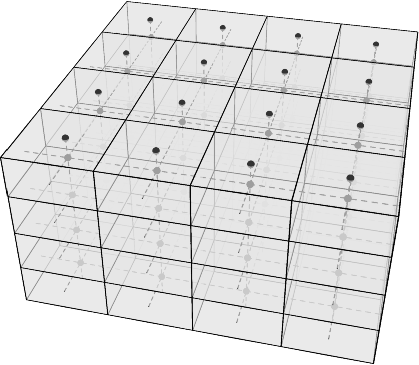
\includegraphics[width=8cm]{spatialgrid.pdf}
  \caption{Spatial grid}
  \label{fig:spatial_grid}
\end{figure}

\begin{align}
  dx &= \frac{x_{\max}-x_{\min}}{n_x} \\ 
  dy &= \frac{y_{\max}-y_{\min}}{n_y} \\ 
  dz &= \frac{z_{\max}-z_{\min}}{n_z}
\end{align}

Then,
\begin{align}
  x_i &= (i-1/2)dx \\
  y_j &= (j-1/2)dy \\
  z_k &= (k-1/2)dz
\end{align}

\subsection{Angular Grid}
\begin{figure}[H]
  \centering
  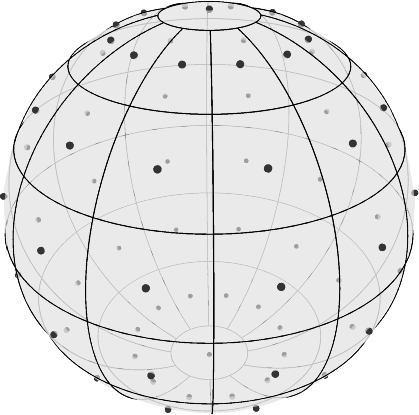
\includegraphics[width=8cm]{angulargrid.pdf}
  \caption{Angular grid}
  \label{fig:angular_grid}
\end{figure}

The azimuthal dimension is unique in that its extreme values are grid centers.
That is,
\begin{align}
  \phi_1 &= 0, \\
  \phi_{n_\phi} &= \pi.
\end{align}

Meanwhile, $\theta$ is similar to the spatial dimensions in that its extreme
values are not grid centers.
Then,
\begin{align}
  d\theta &= \frac{2\pi}{n_\theta}, \\
  d\phi &= \frac{\pi}{n_\phi-1}.
\end{align}

Then,
\begin{align}
  \theta_l = (l-1) d\theta, \\
  \phi_m = (m-1) d\phi
\end{align}

It is also useful to define the edges between angular grid cells as
\begin{alignat}{3}
  \theta_l^e &= (l-1/2) d\theta, &\quad l&=1,\ldots,n_\theta \\
  \phi_m^e &= (m-1/2) d\phi, &\quad m&=1,\ldots,n_\phi-1.
\end{alignat}


As shown in Figure \ref{fig:angular_grid}, $\phi=0$ and $\phi=\pi$, called
the north ($+z$) and south ($-z$) poles respectively, are treated separately.
The total number of angles considered is $n_{\vec{\omega}} = n_\phi n_\theta -
2(n_\theta-1)$.
Since the poles create a non-rectangular angular grid in the sense that
$n_{\vec{\omega}}$ is not the product of two integers, it is advantageous to use
a single variable $p=1,\ldots,n_{\vec{\omega}}$ to index angles $\vec{\omega} =
(\theta, \phi)$ such that $p \in \left\{ 1,\ldots,n_{\vec{\omega}}-2 \right\}$ refers to the interior
of the angular grid, and $p=\left( n_{\vec{\omega}}-1\right)$ and $p=n_{\vec{\omega}}$ refer to the
north and south poles respectively.
The following notation is used.
\begin{align}
  \hat{l}(p) &= \mod(p, n_\theta) + 1 \\
  \hat{m}(p) &= \ceil(p/n_\theta) \\
  \hat{\theta}_p &= \theta_{\hat{l}(p)} \\
  \hat{\phi}_p &= \phi_{\hat{m}(p)}
\end{align}

Thus, it follows that
\begin{equation}
  p = \left( \hat{m}(p)-1\right)n_\theta + \hat{l}(p).
\end{equation}

Accordingly, we define
\begin{equation}
  \hat{p}(l,m) = (m-1)n_\theta + l.
\end{equation}

\subsection{Angular Quadrature}
We assume that all quantities are constant within a spatial-angular grid cell.
We therefore employ the midpoint rule for both spatial and angular integration.

** Need to define $\mathcal{X}$ in this context and write $f$ explicitly as sum
over grid cells.

** Is $d\theta$, etc. for both differential and grid spacing confusing?

\begin{align}
  \int_{4\pi} f(\vec{\omega})\,d\vec{\omega} &= \int_0^{2\pi} \int_0^{\pi} f(\theta, \phi) \sin(\phi)\, d\phi\, d\theta \\
                                             &= \mbox{poles} + \int_0^{2\pi}\int_0^{\pi} \sum_{l=1}^{n_\theta}\sum_{m=2}^{n_\phi-1}\mathcal{X}_l(\theta) \mathcal{X}_m(\phi) f_{\hat{p}(l,m)} \sin(\phi)\, d\phi\, d\theta \\
                                             &= \mbox{poles} + \sum_{l=1}^{n_\theta}\sum_{m=2}^{n_\phi-1}f_{\hat{p}(l,m)}\int_{\theta_l^e}^{\theta_{l+1}^e}\int_{\phi_m^e}^{\phi_{m+1}^e} \sin(\phi)\, d\phi\, d\theta \\
                                             &= \mbox{poles} + d\theta\sum_{l=1}^{n_\theta}\sum_{m=2}^{n_\phi-1} f_{\hat{p}(l,m)}\int_{\phi_m^e}^{\phi_{m+1}^e} \sin(\phi)\, d\phi \\
                                             &= 2\pi\cos(\frac{d\phi}{2})\left( f_{n_{\vec{\omega}}-1}+f_{\vec{\omega}}\right) \\&+ d\theta\sum_{l=1}^{n\theta}\sum_{m=1}^{n\phi} f_{\hat{p}(l,m)}\left( \cos(\phi_m^e)-\cos(\phi_{m+1}^e) \right) \nonumber
\end{align}

Let
\begin{equation}
  \delta_p = \cos(\phi_{\hat{m}(p)}^e)-\cos(\phi_{\hat{m}(p)+1}^e).
\end{equation}

Then,
\begin{equation}
  \int_{4\pi} f(\vec{\omega})\,d\vec{\omega} = 2\pi\cos(\frac{d\phi}{2})\left( f_{n_{\vec{\omega}}-1}+f_{\vec{\omega}}\right) + d\theta\sum_{p=1}^{n_{\vec{\omega}}-2} f_p\delta_p
 \end{equation}


 urface
Note that $0$ is not stored as a grid center in any spatial dimension.
Radiance values for the surface boundary condition are stored
separately as the array $(f_p)$.

\subsection{Discrete Variable Notation}

$L_{ijkp}$, $a_{ijk}$, $f_p$

\section{Finite Difference}

\subsection{Discretization}

For the spatial interior of the domain, we use the 2nd order central difference formula (CD2) to approximate the derivatives, which is
\begin{equation}
    \tag{CD2}
    f'(x) = \frac{f(x+dx)-f(x-dx)}{2dx} + \mathcal{O}(dx^3).
\end{equation}

When applying the PDE on the upper or lower boundary, we use the forward and backward difference (FD2 and BD2) formulas respectively.
Omitting $\mathcal{O}(dx^3)$, we have
\begin{equation}
    \tag{FD2}
    \label{eq:FD2}
    f'(x) = \frac{-3f(x)+2f(x+dx)-f(x+2dx)}{2dx}
\end{equation}
\begin{equation}
    \tag{BD2}
    \label{eq:BD2}
    f'(x) = \frac{3f(x)-2f(x-dx)+f(x-2dx)}{2dx}
\end{equation}

For the upper and lower boundaries, we need an asymmetric finite difference
method.
In general, the Taylor Series of a function $f$ about $x$ is
\begin{equation}
  f'(x+\varepsilon) = \sum_{n=1}^\infty \frac{f^{(n)}(x)}{n!} \varepsilon^n \\
\end{equation}

Truncating after the first few terms, we have
\begin{equation}
  \label{eqn:afd1}
  f'(x+\varepsilon)  = f(x) + f'(x)\varepsilon + \frac{f''(x)}{2}\varepsilon^2 + \mathcal{O}(\varepsilon^3)
\end{equation}

Similarly, replacing $\varepsilon$ with $-\varepsilon/2$ we have
\begin{equation}
  \label{eqn:afd2}
  f'(x-\frac{\varepsilon}{2}) = f(x) - \frac{f'(x)\varepsilon}{2} + \frac{f''(x)\varepsilon^2}{8} + \mathcal{O}(\varepsilon^3).
\end{equation}

Rearranging \eqref{eqn:afd1} produces
\begin{equation}
  \label{eqn:afd3}
  f''(x)\varepsilon^2 = 2f(x+\varepsilon) - 2f(x) - 2f'(x)\varepsilon + \mathcal{O}(\varepsilon^3)
\end{equation}

Combining \eqref{eqn:afd2} with \eqref{eqn:afd3} gives
\begin{align*}
  \varepsilon f'(x) &= 2f(x) - 2f(x-\frac{\varepsilon}{2}) + f''(x)\frac{\varepsilon^2}{8} + \mathcal{O}(\varepsilon^3) \\
                    &= 2f(x) - 2f(x-\frac{\varepsilon}{2}) + \frac{f(x+\varepsilon)}{4} - \frac{f(x)}{4} - \frac{f'(x)\varepsilon}{4} + \mathcal{O}(\varepsilon^3) \\
                    &= \frac{4}{5}\left( 2f(x)-2f(x-\frac{\varepsilon}{2}) + \frac{f(x+\varepsilon)}{4} - \frac{f(x)}{4} \right) + \mathcal{O}(\varepsilon^3)
\end{align*}

Then, dividing by $\varepsilon$ gives
\begin{equation}
  f'(x) = \frac{-8f(x-\frac{\varepsilon}{2}) + 7f(x) + f(x+\varepsilon)}{5\varepsilon} + \mathcal{O}(\varepsilon^2)
\end{equation}

Similarly, substituting $\varepsilon \to -\varepsilon$, we have 
\begin{equation}
  f'(x) = \frac{- f(x-\varepsilon) - 7f(x) + 8f(x+\frac{\varepsilon}{2})}{5\varepsilon} + \mathcal{O}(\varepsilon^2)
\end{equation}


\subsection{Difference Equation}

* Periodic $x,y$

Interior:
\begin{equation}
  \begin{aligned}
    &\frac{L_{i+1,jkp}-L_{i-1,jkp}}{2dx}\sin\hat{\phi}_p\cos\hat{\theta}_p \\
    + &\frac{L_{i,j+1,kp}-L_{i,j-1,kp}}{2dy}\sin\hat{\phi}_p\sin\hat{\theta}_p \\
    + &\frac{L_{ij,k+1,p}-L_{ij,k-1,p}}{2dz}\cos\hat{\phi}_p + (a_{ijk}+b)L_{ijkp} \\
    - &2\pi\cos\left( \frac{d\theta}{2} \right)(L_{ijk,n_{\vec{\omega}}-1}+L_{ijk,n_{\vec{\omega}}}) \\
    - &d\theta \sum_{\substack{p'=1 \\ p' \neq p}}^{n_{\vec{\omega}}-2} L_{ijkp'}\delta_{p'} = 0
  \end{aligned}
\end{equation}

Note that when discretizing the integral, we exclude the $p'=p$ term of the sum.
This is because that term corresponds to ``scattering'' straight ahead
($\abs{\vec{\omega}-\vec{\omega}'}=0$), which is in fact not scattering at all,
but rather transmission.


Surface downwelling (BC):
\begin{equation*}
  \begin{aligned}
    &\frac{L_{i+1,jkp}-L_{i-1,jkp}}{2dx}\sin\hat{\phi}_p\cos\hat{\theta}_p \\
    + &\frac{L_{i,j+1,kp}-L_{i,j-1,kp}}{2dy}\sin\hat{\phi}_p\sin\hat{\theta}_p \\
    + &\frac{-8f_p + 7L_{ijkp} + L_{ij,k+1,p}}{5dz}\cos\hat{\phi}_p  + (a_{ijk}+b)L_{ijkp} \\
    - &2\pi\cos\left( \frac{d\theta}{2} \right)(L_{ijk,n_{\vec{\omega}}-1}+L_{ijk,n_{\vec{\omega}}}) \\
    - &d\theta \sum_{\substack{p'=1 \\ p' \neq p}}^{n_{\vec{\omega}}-2} L_{ijkp'}\delta_{p'} = 0
  \end{aligned}
\end{equation*}

Combining $L_{ijkp}$ terms on the left and moving the boundary condition to the
right gives

\begin{equation}
  \begin{aligned}
    &\frac{L_{i+1,jkp}-L_{i-1,jkp}}{2dx}\sin\hat{\phi}_p\cos\hat{\theta}_p \\
    + &\frac{L_{i,j+1,kp}-L_{i,j-1,kp}}{2dy}\sin\hat{\phi}_p\sin\hat{\theta}_p \\
    + &\frac{L_{ij,k+1,p}}{5dz}\cos\hat{\phi}_p + (a_{ijk} + b +\frac{7}{5dz})L_{ijkp} \\
    - &2\pi\cos\left( \frac{d\theta}{2} \right)(L_{ijk,n_{\vec{\omega}}-1}+L_{ijk,n_{\vec{\omega}}}) \\
    - &d\theta \sum_{\substack{p'=1 \\ p' \neq p}}^{n_{\vec{\omega}}-2} L_{ijkp'}\delta_{p'} = \frac{8f_p}{5dz}.
  \end{aligned}
\end{equation}

Likewise for the bottom boundary condition, we have

\begin{equation}
  \begin{aligned}
    &\frac{L_{i+1,jkp}-L_{i-1,jkp}}{2dx}\sin\hat{\phi}_p\cos\hat{\theta}_p \\
    + &\frac{L_{i,j+1,kp}-L_{i,j-1,kp}}{2dy}\sin\hat{\phi}_p\sin\hat{\theta}_p \\
    - &\frac{L_{ij,k-1,p}}{5dz}\cos\hat{\phi}_p + (a_{ijk} + b -\frac{7}{5dz})L_{ijkp} \\
    - &2\pi\cos\left( \frac{d\theta}{2} \right)(L_{ijk,n_{\vec{\omega}}-1}+L_{ijk,n_{\vec{\omega}}}) \\
    - &d\theta \sum_{\substack{p'=1 \\ p' \neq p}}^{n_{\vec{\omega}}-2} L_{ijkp'}\delta_{p'} = 0.
  \end{aligned}
\end{equation}

Now, for upwelling light at the first depth layer (non-BC), we apply FD2.
\begin{equation}
  \begin{aligned}
    &\frac{L_{i+1,jkp}-L_{i-1,jkp}}{2dx}\sin\hat{\phi}_p\cos\hat{\theta}_p \\
    + &\frac{L_{i,j+1,kp}-L_{i,j-1,kp}}{2dy}\sin\hat{\phi}_p\sin\hat{\theta}_p \\
    + &\frac{-3L_{ijkp} + 2L_{ij,k+1,p} - L_{ij,k+2,p}}{2dz}\cos\hat{\phi}_p + (a_{ijk}+b)L_{ijkp} \\
    - &2\pi\cos\left( \frac{d\theta}{2} \right)(L_{ijk,n_{\vec{\omega}}-1}+L_{ijk,n_{\vec{\omega}}}) \\
    - &d\theta \sum_{\substack{p'=1 \\ p' \neq p}}^{n_{\vec{\omega}}-2} L_{ijkp'}\delta_{p'} = 0
  \end{aligned}
\end{equation}

Grouping $L_{ijkp}$ terms gives
\begin{equation}
  \begin{aligned}
    &\frac{L_{i+1,jkp}-L_{i-1,jkp}}{2dx}\sin\hat{\phi}_p\cos\hat{\theta}_p \\
    + &\frac{L_{i,j+1,kp}-L_{i,j-1,kp}}{2dy}\sin\hat{\phi}_p\sin\hat{\theta}_p \\
    + &\frac{2L_{ij,k+1,p} - L_{ij,k+2,p}}{2dz}\cos\hat{\phi}_p + \left(a_{ijk}+b - 3\frac{\cos\hat\phi_p}{2dz} \right)L_{ijkp} \\
    - &2\pi\cos\left( \frac{d\theta}{2} \right)(L_{ijk,n_{\vec{\omega}}-1}+L_{ijk,n_{\vec{\omega}}}) \\
    - &d\theta \sum_{\substack{p'=1 \\ p' \neq p}}^{n_{\vec{\omega}}-2} L_{ijkp'}\delta_{p'} = 0
  \end{aligned}
\end{equation}

Similarly, for downwelling light at the lowest depth layer, we have
\begin{equation}
  \begin{aligned}
    &\frac{L_{i+1,jkp}-L_{i-1,jkp}}{2dx}\sin\hat{\phi}_p\cos\hat{\theta}_p \\
    + &\frac{L_{i,j+1,kp}-L_{i,j-1,kp}}{2dy}\sin\hat{\phi}_p\sin\hat{\theta}_p \\
    + &\frac{-2L_{ij,k-1,p} + L_{ij,k-2,p}}{2dz}\cos\hat{\phi}_p + \left(a_{ijk}+b + 3\frac{\cos\hat\phi_p}{2dz} \right)L_{ijkp} \\
    - &2\pi\cos\left( \frac{d\theta}{2} \right)(L_{ijk,n_{\vec{\omega}}-1}+L_{ijk,n_{\vec{\omega}}}) \\
    - &d\theta \sum_{\substack{p'=1 \\ p' \neq p}}^{n_{\vec{\omega}}-2} L_{ijkp'}\delta_{p'} = 0
  \end{aligned}
\end{equation}

\subsection{Structure of Linear System}

Describe layout of matrix.

Number of rows/columns: $n_xn_yn_zn_{\vec{\omega}}$

Number of nonzero RHS entries: $n_xn_yn_z$

** Table with number of nonzero matrix entries in each type of row (interior,
exterior-BC, exterior non-BC)

Number of nonzero matrix entries: $n_xn_yn_{\vec{\omega}} \left[n_z(n_{\vec{\omega}}+6)-1 \right]$

\section{GMRES}
GMRES is a Krylov Subspace method. These work like this. Here's what's special
about GMRES. Advantages. Drawbacks. Not practical for running in SINMOD.

\section{Numerical Asymptotics}

\subsection{Ray Tracing Algorithm}
\subsubsection{Extract values along path}

In order to evaluate a path integral through the previously described grid, it
is first necessary to construct a one-dimensional piecewise constant integrand
which is discontinuous at unevenly spaced points corresponding to the
intersections between the path and edges in the spatial grid.

Consider a grid center $\vec{x_1} = (x_1,y_1,z_1)$ and a corresponding path $\vec{l}(\vec{x_1}, \vec{\omega}, s)$.
To find the location of discontinuities in the itegrand, we first calculate the
distance from its origin, $\vec{x_0}(\vec{x_1}, \vec{\omega}) = (x_0, y_0, z_0)$ to grid edges in each dimension
separately.


** THIS NOTATION IS OVERLOADED **

Given
\begin{align}
  x_i &= x_0 + s_i^x/\tilde{s}(x_1-x_0) \\
  y_j &= y_0 + s_j^y/\tilde{s}(y_1-y_0) \\
  z_k &= z_0 + s_k^z/\tilde{s}(z_1-z_0)
\end{align}

we have
\begin{align}
  s_i^x &= \tilde{s}\frac{x_i-x_0}{x_1-x_0} \\
  s_i^y &= \tilde{s}\frac{y_i-y_0}{y_1-y_0} \\
  s_i^z &= \tilde{s}\frac{z_i-z_0}{z_1-z_0} \\
\end{align}

Then, move to the adjacent grid cell in the dimension which requires the shortes
step to reach an edge. Save $ds$ of the path through this cell. Also save abs.
coef. and source.
** Definitely needs more work**

- absorption coefficient ($\tilde{a}(s)$)

- effective source ($g_n(s)$)

\subsubsection{Ray integral}

Here are the equations for calculating the double integral over ray paths
required for the asymptotics. It will hopefully make more sense once I add words
to accompany the symbols.

Let
\begin{align}
  g_n(s) &= \sum_{i=1}^{N-1}g_{ni}\mathcal{X}_i(s) \\
  \tilde{a}(s) &= \sum_{i=1}^{N-1}\tilde{a}_{i}\mathcal{X}_i(s) \\
\end{align}

and
\begin{equation}
  \mathcal{X}_i(s) = \begin{cases}
    1, & a_I \leq s < s_{i+1} \\
    0, & \mbox{otherwise}
    \end{cases}
\end{equation}

and $\left\{s_i\right\}_{i=1}^N$ is increasing.

Let $ds_i = s_{i+1} - s_i$.

Let $\hat{i}(s) = \min\left\{ i \in \{1,\ldots,N\} : s_i>s \right\}$.
Let $\tilde{d}(s) = s_{\hat{i}(s)}-s$.

We have $s_1 = 0$ and $s_N = \tilde{s}$.


\begin{align}
  u_n(\tilde{s}) &= \int_0^{\tilde{s}}g_n(s')\exp\left( -\int_{s''}^{s'}\tilde{a}(s'')\,ds'' \right)\, ds' \\
  &= \int_0^{s_N} \sum_{i=1}^{N-1}g_{ni}\mathcal{X}_i(s') \exp\left( -\int_{s''}^{s'}\sum_{j=1}^{N-1}\tilde{a}_{j}\mathcal{X}_j(s'')\,ds'' \right)\, ds' \\
  &= \sum_{i=1}^{N-1}g_{ni}\int_0^{s_N} \mathcal{X}_i(s') \exp\left( -\sum_{j=1}^{N-1}\tilde{a}_{j}\int_{s''}^{s'}\mathcal{X}_j(s'')\,ds'' \right)\, ds' \\
  &= \sum_{i=1}^{N-1}g_{ni}\int_{s_i}^{s_{i+1}}  \exp\left(-\tilde{a}_{\hat{i}(s')-1}\tilde{d}(s') -\sum_{j=\hat{i}(s')}^{N-1}\tilde{a}_{j}ds_j\right)\, ds' \\
  &= \sum_{i=1}^{N-1}g_{ni}\int_{s_i}^{s_{i+1}}  \exp\left(-\tilde{a}_{i}(s_{i+1}-s') -\sum_{j=i+1}^{N-1}\tilde{a}_{j}ds_j\right)\, ds'
\end{align}

Let
\begin{equation}
  b_i = -\tilde{a}_{i}s_{i+1} - \sum_{j=i+1}^{N-1}\tilde{a}_{j}ds_j.
\end{equation}

Then,
\begin{equation}
  u_n(\tilde{s}) = \sum_{i=1}^{N-1}g_{ni}\int_{s_i}^{s_{i+1}}  \exp\left(\tilde{a}_{i}s' +b_i\right)\, ds'
\end{equation}

Let
\begin{align}
  d_i &= \int_{s_i}^{s_{i+1}}  \exp\left(\tilde{a}_{i}s' +b_i\right)\, ds' \\
    &= \begin{cases}
    ds_i \exp(b_i), & \tilde{a} = 0 \\
      \left( \exp(\tilde{a}_i s_{i+1}) - \exp(\tilde{a}_i s_i) \right)/\tilde{a}_i, & \mbox{otherwise}
    \end{cases}
\end{align}

Then,
\begin{equation}
  u_n(\tilde{s}) = \sum_{i=1}^{N-1} g_{ni}d_i
\end{equation}